\documentclass[preprint,12pt,aps,pra,showkeys,amsmath,amssymb,superscriptaddress,floatfix]{revtex4-2}
\usepackage[T1]{fontenc}
\usepackage[utf8]{inputenc}
\usepackage{amsmath,amssymb,amsthm,mathtools,mathrsfs}
\usepackage{microtype,booktabs,enumitem}
\usepackage{xcolor,tikz,etoolbox}
\usepackage[skins,breakable]{tcolorbox}
\usepackage{needspace}
% Keep diagram geometry independent of REVTeX preprint body spacing.
\AtBeginEnvironment{tikzpicture}{\linespread{1}\selectfont}
\usetikzlibrary{arrows.meta,positioning,calc,fit,decorations.pathreplacing}
\usepackage{graphicx}
\usepackage{hyperref}

\definecolor{MMBlue}{RGB}{0,82,155}
\definecolor{MMOrange}{RGB}{200,80,0}
\tikzset{
 mmnode/.style={draw=MMBlue,rounded corners=2pt,fill=MMBlue!4,align=left,execute at begin node={\raggedright},text width=5cm,font=\fontsize{10}{12}\selectfont,inner sep=6pt},
 mmimport/.style={mmnode,draw=black!65,fill=black!4},
 mmcandidate/.style={mmnode,draw=MMOrange,dashed,fill=MMOrange!5},
 mmrejected/.style={mmnode,draw=black,densely dotted,fill=black!8},
 mmproof/.style={->,thick,MMBlue},
 mmflow/.style={->,semithick,black!70},
 mmrepair/.style={->,dashed,thick,MMOrange},
 mmcandidatearrow/.style={->,dashed,semithick,MMOrange},
 mmnote/.style={font=\scriptsize,fill=white,inner sep=2pt,align=center}}

\usepackage[section]{placeins}
\setlength{\emergencystretch}{3em}
\setlist{itemsep=3pt,topsep=4pt}
\newtheorem{theorem}{Theorem}[section]
\newtheorem{proposition}[theorem]{Proposition}
\newtheorem{lemma}[theorem]{Lemma}
\newtheorem{corollary}[theorem]{Corollary}
\theoremstyle{definition}
\newtheorem{definition}[theorem]{Definition}
\newtheorem{example}[theorem]{Example}
\theoremstyle{remark}
\newtheorem{remark}[theorem]{Remark}
% Avoid isolated statement headings and single-line paragraph fragments.
\BeforeBeginEnvironment{theorem}{\Needspace{6\baselineskip}}
\BeforeBeginEnvironment{definition}{\Needspace{5\baselineskip}}
\BeforeBeginEnvironment{proposition}{\Needspace{5\baselineskip}}
\BeforeBeginEnvironment{lemma}{\Needspace{5\baselineskip}}
\BeforeBeginEnvironment{corollary}{\Needspace{5\baselineskip}}
\clubpenalty=5000
\widowpenalty=5000
\newcommand{\R}{\mathbb R}\newcommand{\Z}{\mathbb Z}\newcommand{\N}{\mathbb N}
\newcommand{\Pa}{\operatorname{Pa}}\newcommand{\Desc}{\operatorname{Desc}}
\newcommand{\cl}{\operatorname{cl}}\newcommand{\cost}{\operatorname{cost}}
\newcommand{\status}{\operatorname{status}}
% Faculty cards: a visual rail groups the five faculties within one agent.
% The rail has no arrowhead and does not represent a proof dependency.
\newcommand{\mmfacultybadge}[1]{%
 \node[circle,draw=MMBlue,line width=1pt,fill=white,
 minimum size=7mm,inner sep=0pt,font=\sffamily\small\bfseries,text=MMBlue]
 at ([xshift=15pt,yshift=-15pt]frame.north west) {#1};}
\newcommand{\mmfacultyrail}{%
 \draw[MMBlue!80,line width=1pt]
 ([xshift=15pt,yshift=2pt]frame.north west)--
 ([xshift=15pt,yshift=-2pt]frame.south west);}
\newtcolorbox{mmfacultybox}[2]{enhanced,breakable,
 colback=MMBlue!4,colframe=MMBlue!4,boxrule=0pt,arc=3pt,
 left=39pt,right=9pt,top=4pt,bottom=4pt,
 before skip=2pt,after skip=2pt,
 fontupper=\small\linespread{1.1}\selectfont,
 overlay unbroken={\mmfacultyrail\mmfacultybadge{#1}},
 overlay first={\mmfacultyrail\mmfacultybadge{#1}},
 overlay middle={\mmfacultyrail},overlay last={\mmfacultyrail}}
\newcommand{\mmfaculty}[3]{%
 \begin{mmfacultybox}{#1}{#2}
 {\sffamily\bfseries\color{MMBlue}#2}\par\smallskip #3
 \end{mmfacultybox}}
\newcommand{\agent}[9]{%
 \Needspace{8\baselineskip}
 \subsubsection{#1}
 \noindent\textbf{Object.} #2\par
 \noindent\textbf{Role.} #3\par\smallskip
 \mmfaculty{E}{Ego}{#4}
 \mmfaculty{M}{Memory}{#5}
 \mmfaculty{I}{Intellect}{#6}
 \mmfaculty{S}{Sense}{#7}
 \mmfaculty{A}{Action}{#8}
 \smallskip\noindent #9\par}

\usepackage{longtable,array,calc}
\providecommand{\tightlist}{\setlength{\itemsep}{2pt}\setlength{\parskip}{0pt}}
\makeatletter
\def\frontmatter@abstract@produce{\par\addvspace{\frontmatter@preabstractspace}%
\begingroup\prep@absbox\unvbox\absbox\post@absbox\endgroup
\addvspace{\frontmatter@postabstractspace}}
\makeatother
\newcommand{\field}[2]{\par\smallskip\noindent\textbf{#1.} #2\par}
\setlength{\emergencystretch}{5em}
\AtBeginEnvironment{verbatim}{\small\linespread{1.0}\selectfont}


\hypersetup{colorlinks=true,linkcolor=MMBlue,urlcolor=MMBlue,pdfauthor={Dibakar Sigdel}}

\begin{document}

\title{Affine Polynomial Maps and Coordinate-Ring Duality\\[4pt]\large An End-to-End Meta-Math Walkthrough}

\author{Dibakar Sigdel}

\affiliation{Mindverse Computing LLC, Lynnwood, WA 98087, USA}

\date{October 2026}

\begin{abstract}

The images of the coordinate functions determine the point map.
Relations in the source coordinate ring guarantee that the reconstructed
point lies in the intended target. The report presents the target
theorem, declared imports, a dependency graph, five-faculty node
contracts, a continuous proof, a worked example, and a hypothesis-repair
audit. It is an authored mathematical exposition, not a deployed-agent
transcript or a formal proof-assistant certificate.

\end{abstract}\maketitle\linespread{1.12}\selectfont

\noindent\textbf{AG-05 / Algebraic Geometry / Report v1}

\section{Target and import contract}

\begin{theorem}

For affine algebraic sets \(X\subset k^n\) and \(Y\subset k^m\),
polynomial maps \(F:X\to Y\) are in bijection with unital \(k\)-algebra
homomorphisms \(\phi:k[Y]\to k[X]\) via pullback \(F^*(h)=h\circ F\).
Composition is reversed. A polynomial map is an isomorphism with
polynomial inverse if and only if its pullback is a \(k\)-algebra
isomorphism. Here polynomial maps mean maps whose coordinate functions
are restrictions of polynomials.

\end{theorem}

\subsection{Foundations and permitted imports}

Use quotient rings, the vanishing ideal \(I(X)\) of the actual point
set, and \(V(I(X))=X\) for an algebraic set: if \(X=V(S)\), then
\(S\subset I(X)\) gives \(V(I(X))\subset X\), while the reverse
inclusion is definitional. Constants are fixed by a \(k\)-algebra map.
No Nullstellensatz or algebraic closure is necessary for this
formulation.

\clearpage\section{Node interaction workflow}

\begin{center}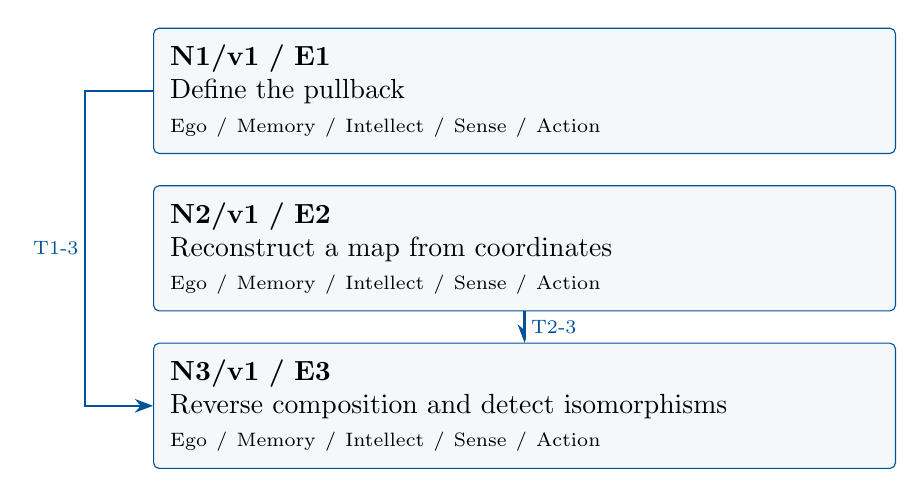
\begin{tikzpicture}[>=Stealth,x=1cm,y=1cm]

\node[mmnode,text width=9cm,minimum height=1.25cm] (N1) at (0,0.0) {\textbf{N1/v1 / E1}\\Define the pullback\\{\scriptsize Ego / Memory / Intellect / Sense / Action}};

\node[mmnode,text width=9cm,minimum height=1.25cm] (N2) at (0,-2.0) {\textbf{N2/v1 / E2}\\Reconstruct a map from coordinates\\{\scriptsize Ego / Memory / Intellect / Sense / Action}};

\node[mmnode,text width=9cm,minimum height=1.25cm] (N3) at (0,-4.0) {\textbf{N3/v1 / E3}\\Reverse composition and detect isomorphisms\\{\scriptsize Ego / Memory / Intellect / Sense / Action}};

\draw[mmproof] (N1.west) -- (-5.58,0) -- node[mmnote,left] {T1-3} (-5.58,-4) -- (N3.west);

\draw[mmproof] (N2.south) -- node[mmnote,right] {T2-3} (N3.north);

\end{tikzpicture}\end{center}

Each box is one mathematical agent containing all five faculties. Blue
arrows carry the versioned exports listed below. The layout gives a
reading order; only drawn arrows assert dependencies. Diagnostic repair
is separate from the proof DAG.

\subsection{Versioned evidence-transfer ledger}

\begingroup\small\linespread{1.05}\selectfont

\Needspace{5\baselineskip}\field{T1-3: N1/E1/v1 to N3}{\(F^*:k[Y]\to k[X]\) is a well-defined unital \(k\)-algebra
homomorphism.}

\field{Receiving activity}{N3.1}

\field{Compatibility}{E1/v1 and E2/v1; maps \(X\xrightarrow{F}Y\xrightarrow{G}Z\). Check: The
arrow directions reverse: \((G\circ F)^*=F^*\circ G^*\).}

\Needspace{5\baselineskip}\field{T2-3: N2/E2/v1 to N3}{There is a unique polynomial map \(F:X\to Y\) with \(F^*=\phi\).}

\field{Receiving activity}{N3.1}

\field{Compatibility}{E1/v1 and E2/v1; maps \(X\xrightarrow{F}Y\xrightarrow{G}Z\). Check: The
arrow directions reverse: \((G\circ F)^*=F^*\circ G^*\).}

\endgroup

\clearpage\section{Agent roles and five-faculty activities}\begingroup\small\linespread{1.05}\selectfont\setlist{itemsep=1pt,topsep=2pt}

\subsection{N1/v1: Define the pullback}

\field{Object and role}{Compose representative polynomials and show the result is independent of
representatives. \textbf{Local obligation:} \(F^*:k[Y]\to k[X]\) is a
well-defined unital \(k\)-algebra homomorphism.}

\field{Inputs}{A polynomial map \(F=(F_1,\ldots,F_m):X\to Y\).}

\mmfaculty{E}{Ego}{Publish E1/v1 only after establishing this obligation:
\(F^*:k[Y]\to k[X]\) is a well-defined unital \(k\)-algebra
homomorphism.}

\mmfaculty{M}{Memory}{A polynomial map \(F=(F_1,\ldots,F_m):X\to Y\). Retain the stated
assumptions and import versions.}

\mmfaculty{I}{Intellect}{Compose representative polynomials and show the result is independent of
representatives.}

\mmfaculty{S}{Sense}{Two representatives equal on \(Y\) must remain equal after composition
because \(F(X)\subset Y\).}

\mmfaculty{A}{Action}{Carry out activities N1.1--N1.2 below, retaining each calculation and
construction as evidence.}

\smallskip\noindent\textbf{Numbered mathematical activities}

\begin{enumerate}[label=N1.\arabic*,leftmargin=3.4em]

\item For a polynomial \(h\) in the \(Y\) coordinates, substitute the
polynomial coordinates of \(F\) to obtain a polynomial function on
\(X\). If \(h-h'\in I(Y)\), then \((h-h')(F(x))=0\) for every
\(x\in X\), so the resulting classes in \(k[X]\) agree.

\item Composition preserves addition, multiplication, the constant \(1\), and
each scalar in \(k\). It also does not depend on the representatives
chosen for \(F_i\), because those representatives agree pointwise on
\(X\). This proves the pullback assertion.

\end{enumerate}

\field{Export E1/v1}{\(F^*:k[Y]\to k[X]\) is a well-defined unital \(k\)-algebra
homomorphism.}

\field{Acceptance gate}{Two representatives equal on \(Y\) must remain equal after composition
because \(F(X)\subset Y\).}

\field{Targeted repair}{If composition is defined before target membership is checked, verify
\(F(X)\subset Y\); otherwise relations in \(I(Y)\) need not vanish.
Withhold this export and recheck its descendants after a versioned
correction.}

\clearpage

\subsection{N2/v1: Reconstruct a map from coordinates}

\field{Object and role}{Choose representatives for the images of coordinate classes and verify
every defining relation of \(Y\). \textbf{Local obligation:} There is a
unique polynomial map \(F:X\to Y\) with \(F^*=\phi\).}

\field{Inputs}{A unital \(k\)-algebra homomorphism \(\phi:k[Y]\to k[X]\).}

\mmfaculty{E}{Ego}{Publish E2/v1 only after establishing this obligation: There is a unique
polynomial map \(F:X\to Y\) with \(F^*=\phi\).}

\mmfaculty{M}{Memory}{A unital \(k\)-algebra homomorphism \(\phi:k[Y]\to k[X]\). Retain the
stated assumptions and import versions.}

\mmfaculty{I}{Intellect}{Choose representatives for the images of coordinate classes and verify
every defining relation of \(Y\).}

\mmfaculty{S}{Sense}{The images are elements of the quotient \(k[X]\), so changing
representatives must not change the point map.}

\mmfaculty{A}{Action}{Carry out activities N2.1--N2.2 below, retaining each calculation and
construction as evidence.}

\smallskip\noindent\textbf{Numbered mathematical activities}

\begin{enumerate}[label=N2.\arabic*,leftmargin=3.4em]

\item Let \(\bar y_j\) be the coordinate classes of \(k[Y]\). Choose
polynomials \(p_j\) representing \(\phi(\bar y_j)\), and set
\(F(x)=(p_1(x),\ldots,p_m(x))\). Representatives differing by \(I(X)\)
give the same map.

\item For every \(h\in I(Y)\), \(h(\bar y_1,\ldots,\bar y_m)=0\) in \(k[Y]\).
Applying \(\phi\) gives \(h(p_1,\ldots,p_m)\in I(X)\), hence
\(F(x)\in V(I(Y))=Y\). On all coordinate classes \(F^*\) agrees with
\(\phi\), and these classes and constants generate \(k[Y]\), so
agreement holds everywhere. The coordinate images also force uniqueness.

\end{enumerate}

\field{Export E2/v1}{There is a unique polynomial map \(F:X\to Y\) with \(F^*=\phi\).}

\field{Acceptance gate}{The images are elements of the quotient \(k[X]\), so changing
representatives must not change the point map.}

\field{Targeted repair}{If arbitrary polynomial representatives are used without checking
relations, apply \(\phi\) to every relation in \(I(Y)\) before claiming
target membership. Withhold this export and recheck its descendants
after a versioned correction.}

\clearpage

\subsection{N3/v1: Reverse composition and detect isomorphisms}

\field{Object and role}{Compute compositions on functions and use uniqueness of the recovered
map. \textbf{Local obligation:} Pullback gives the stated bijection,
reverses composition, and identifies polynomial isomorphisms with
algebra isomorphisms.}

\field{Inputs}{E1/v1 and E2/v1; maps \(X\xrightarrow{F}Y\xrightarrow{G}Z\). Incoming
proof exports: E1/v1 at N3.1, E2/v1 at N3.1.}

\mmfaculty{E}{Ego}{Publish E3/v1 only after establishing this obligation: Pullback gives
the stated bijection, reverses composition, and identifies polynomial
isomorphisms with algebra isomorphisms.}

\mmfaculty{M}{Memory}{E1/v1 and E2/v1; maps \(X\xrightarrow{F}Y\xrightarrow{G}Z\). Incoming
proof exports: E1/v1 at N3.1, E2/v1 at N3.1. Retain the stated
assumptions and import versions.}

\mmfaculty{I}{Intellect}{Compute compositions on functions and use uniqueness of the recovered
map.}

\mmfaculty{S}{Sense}{The arrow directions reverse: \((G\circ F)^*=F^*\circ G^*\).}

\mmfaculty{A}{Action}{Carry out activities N3.1--N3.2 below, retaining each calculation and
construction as evidence.}

\smallskip\noindent\textbf{Numbered mathematical activities}

\begin{enumerate}[label=N3.\arabic*,leftmargin=3.4em]

\item For a function \(h\) on \(Z\),
\((G\circ F)^*h=h\circ G\circ F=F^*(G^*h)\). Identity maps pull back to
identity homomorphisms. E1 and E2 are inverse constructions, giving the
bijection.

\item If \(F\) has polynomial inverse \(G\), the composition identities show
that \(F^*\) and \(G^*\) are inverse. Conversely if \(F^*\) is
invertible, E2 realizes its inverse as \(G^*\) for a polynomial map
\(G:Y\to X\). Both composite pullbacks are identities; uniqueness in E2
forces \(G\circ F=\mathrm{id}_X\) and \(F\circ G=\mathrm{id}_Y\).

\end{enumerate}

\field{Export E3/v1}{Pullback gives the stated bijection, reverses composition, and
identifies polynomial isomorphisms with algebra isomorphisms.}

\field{Acceptance gate}{The arrow directions reverse: \((G\circ F)^*=F^*\circ G^*\).}

\field{Targeted repair}{If composition order is reversed incorrectly, evaluate both sides on one
function and rebuild the domain/codomain chain. Withhold this export and
recheck its descendants after a versioned correction.}

\endgroup\clearpage\section{Continuous mathematical proof}\label{sec:proof}

\subsection{N1 --- Define the pullback}\label{n1-define-the-pullback}

\begin{enumerate}
\def\labelenumi{\arabic{enumi}.}
\item
  \textbf{N1.1.} For a polynomial \(h\) in the \(Y\) coordinates,
  substitute the polynomial coordinates of \(F\) to obtain a polynomial
  function on \(X\). If \(h-h'\in I(Y)\), then \((h-h')(F(x))=0\) for
  every \(x\in X\), so the resulting classes in \(k[X]\) agree.
\item
  \textbf{N1.2.} Composition preserves addition, multiplication, the
  constant \(1\), and each scalar in \(k\). It also does not depend on
  the representatives chosen for \(F_i\), because those representatives
  agree pointwise on \(X\). This proves the pullback assertion.
\end{enumerate}

\subsection{N2 --- Reconstruct a map from
coordinates}\label{n2-reconstruct-a-map-from-coordinates}

\begin{enumerate}
\def\labelenumi{\arabic{enumi}.}
\item
  \textbf{N2.1.} Let \(\bar y_j\) be the coordinate classes of \(k[Y]\).
  Choose polynomials \(p_j\) representing \(\phi(\bar y_j)\), and set
  \(F(x)=(p_1(x),\ldots,p_m(x))\). Representatives differing by \(I(X)\)
  give the same map.
\item
  \textbf{N2.2.} For every \(h\in I(Y)\),
  \(h(\bar y_1,\ldots,\bar y_m)=0\) in \(k[Y]\). Applying \(\phi\) gives
  \(h(p_1,\ldots,p_m)\in I(X)\), hence \(F(x)\in V(I(Y))=Y\). On all
  coordinate classes \(F^*\) agrees with \(\phi\), and these classes and
  constants generate \(k[Y]\), so agreement holds everywhere. The
  coordinate images also force uniqueness.
\end{enumerate}

\subsection{N3 --- Reverse composition and detect
isomorphisms}\label{n3-reverse-composition-and-detect-isomorphisms}

\begin{enumerate}
\def\labelenumi{\arabic{enumi}.}
\item
  \textbf{N3.1.} For a function \(h\) on \(Z\),
  \((G\circ F)^*h=h\circ G\circ F=F^*(G^*h)\). Identity maps pull back
  to identity homomorphisms. E1 and E2 are inverse constructions, giving
  the bijection.
\item
  \textbf{N3.2.} If \(F\) has polynomial inverse \(G\), the composition
  identities show that \(F^*\) and \(G^*\) are inverse. Conversely if
  \(F^*\) is invertible, E2 realizes its inverse as \(G^*\) for a
  polynomial map \(G:Y\to X\). Both composite pullbacks are identities;
  uniqueness in E2 forces \(G\circ F=\mathrm{id}_X\) and
  \(F\circ G=\mathrm{id}_Y\).
\end{enumerate}

\hfill$\square$

\section{Worked orchestration}

Over \(k=\mathbb C\), for the parabola \(Y=V(y-x^2)\), the map
\(F:\mathbb A^1\to Y\), \(t\mapsto(t,t^2)\), induces
\(F^*:k[x,y]/(y-x^2)\to k[t]\) with \(x\mapsto t\), \(y\mapsto t^2\).
Its inverse sends \(t\) to the class of \(x\). The corresponding
geometric inverse is \((x,y)\mapsto x\). Both compositions are
explicitly identities.

\subsection{Boundary and hypothesis audit}

A pointwise bijective polynomial map need not be an isomorphism. Over an
algebraically closed field of characteristic \(p>0\), \(t\mapsto t^p\)
is bijective: roots exist and \((a-b)^p=0\) forces equality. Its
pullback \(k[t]\to k[t]\), \(t\mapsto t^p\), is not surjective because
\(t\) is absent from \(k[t^p]\).

\section{Illustrative failure and repair}

The following is an authored diagnostic scenario. Changed assumptions
define a new contract; they do not retroactively prove the original
statement.

\subsection{Rejected argument, diagnosis, and correction}
\textbf{Rejected final export:} every bijective polynomial map has a
polynomial inverse. \textbf{Sense witness:} Frobenius on the affine line
in characteristic \(p\). \textbf{Diagnosis:} Ego promoted a
set-theoretic property to an algebraic one. \textbf{Repair:} use the
actual criterion that the pullback is an algebra isomorphism, as proved
in N3. This rejects a stronger claim while preserving the exact §1
theorem; bijectivity alone remains insufficient.

\subsection{Publication and reuse}
The corrected export retains its explicit assumptions. A hypothetical
revision receives a new version, and each consuming activity is
rechecked; this scenario is not a recorded runtime event. \textbf{Next
direction:} Extend this affine viewpoint to gluing local coordinate
descriptions, while keeping regular maps and pointwise bijections
distinct.

\par\medskip\begingroup\small\linespread{1.0}\selectfont\noindent\textbf{Provenance.} This authored proof is complete relative to its declared imports. Reuse
each export with its assumptions, proof, and version. The original
Markdown remains available for comparison.
\par\endgroup

\par\smallskip\begingroup\small\linespread{1.0}\selectfont\noindent\textbf{Further reading.} \href{https://www.jmilne.org/math/CourseNotes/ag.html}{J. S. Milne,
Algebraic Geometry}, chapters on commutative algebra, algebraic sets,
and affine varieties; \href{https://www.jmilne.org/math/}{author's
mathematics site}.\par\endgroup

\end{document}
